\documentclass[12pt,a4paper]{article}
\usepackage[utf8]{inputenc}
\usepackage[russian]{babel}
\usepackage[OT1]{fontenc}
\usepackage{graphicx}
\usepackage{calc}
\usepackage[margin=15mm]{geometry}
\usepackage{cmap}

% условие без картинки
\newcommand{\task}[2]{
\hrule
\hbox to \textwidth {%
     \vrule
\parbox[t]{0.04\textwidth}{\smallskip \centering #1}%
     \vrule%
\hfill%
     \parbox[t]{0.93\textwidth}{\smallskip #2 \smallskip}\hfill%
\vrule
}
\hrule
    \pagebreak[2]
}

\newlength{\h}
\newsavebox{\taskbox}
\newlength{\x}
\newsavebox{\pictbox}

% условие с картинкой (картинка выравнивается по центру)
\newcommand{\taskpic}[3]{
\savebox{\taskbox}{\parbox[t]{0.93\textwidth-4.3cm}{\smallskip #2 \smallskip}}
\savebox{\pictbox}{\parbox[t]{4cm}{\smallskip \centering
     \vspace{0pt} #3 \smallskip}}
\h=\ht\taskbox
\advance\h\dp\taskbox
\x=\ht\pictbox
\advance\x\dp\pictbox
\hrule
\hbox to \textwidth {%
\vrule\parbox[t][\maxof{\h}{\x}][t]{0.04\textwidth}{ \smallskip
     \centering #1 }\vrule%
\hfill\parbox[t][\maxof{\h}{\x}][t]{0.93\textwidth-4.3cm}{\smallskip #2
     \smallskip}\hfill\vrule%
\hfill\parbox[t][\maxof{\h}{\x}][c]{4cm}{\hfil #3 \hfil}\hfill\vrule
}
\hrule
\pagebreak[2]
}
\pagestyle{empty}
\graphicspath{ {images/} }

\begin{document}
\begin{center}
\begin{Large}
\textsc{ГЦФО. 9 класс. 2014/15.}
\end{Large}
\end{center}
\task{12}{Рядом стоят две пушки, из которых можно стрелять теннисными мячиками под любым углом к горизонту с начальной скоростью $v=20$~м/с. Из пушек одновременно стреляют в бубен, находящийся на расстоянии $L=20$~м по горизонтали, однако удары мячиков о бубен происходят не одновременно. Найдите время между ударами. Расстоянием между пушками, размером бубна, а также сопротивлением воздуха пренебречь. Ускорение свободного падения $g=10$~м/с$^2$.}
\taskpic{13}{Два одинаковых бруса скрепили за середины торцов одинаковыми нерастяжимыми нитями и положили на угол стола (см. рис.). Торцы выступают за края столешницы так, что нити не касаются стола. Коэффициент трения о вертикальную поверхность стола в 3~раза больше, чем о горизонтальную. Известно, что если поставить систему с начальным углом нити к горизонтали $\alpha < 45^\circ$ (см. рис.), то бруски начнут двигаться, тогда как если в начальный момент $\alpha \geqslant 45^\circ$, то система остается неподвижной. Найдите коэффициент трения о горизонтальную поверхность.}{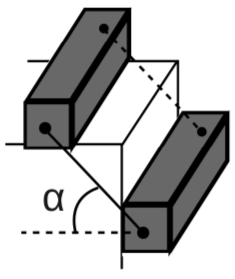
\includegraphics[width=3cm]{13}}
\taskpic{14}{B системе, изображенной на рисунке, пружины имеют жесткости $k_1=100$~Н/м и $k_2=200$ Н/м. К нижнему блоку подвешивают груз массой $M=8$~кг. Система приходит в равновесие. На сколько сместился нижний блок? Пружины, нити и блоки невесомы. Нити нерастяжимы. Ускорение свободного падения $g=10$~м/c$^2$.}{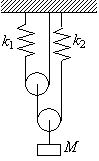
\includegraphics[width=2.5cm]{14}}
\taskpic{15}{На гладкой наклонной плоскости, составляющей с горизонтом угол $\alpha=30^\circ$, расположен массивный клин (см. рис.). На верхней горизонтальной поверхности клина лежит маленькая легкая шайба. Клин отпускают, и он начинает свободно соскальзывать вниз.
\begin{enumerate}
\item Определите величину и направление ускорения движения шайбы относительно наклонной плоскости.
\item Как выглядит движение шайбы в системе отсчета, связанной с клином?
\end{enumerate}
Масса шайбы много меньше массы клина. Трением пренебречь.}{
\begin{tikzpicture}
\draw[thick] (0,1.5)--(3,0);
\draw[thick,dashed] (0.5,0.5)--(2,0.5);
\filldraw[thick,fill=gray] (0.5,1.27)--(2.5,0.27)--(2.5,1.27)--cycle;
\filldraw[fill=black] (1.6,1.28) rectangle (1.8,1.38);
\draw[thick] (1.5,0.5) arc (180:153.5:0.5) node[midway,left] {$\alpha$};
\end{tikzpicture}
}
\taskpic{16}{Три одинаковых бревна, имеющих форму цилиндра, сложены так, как показано на рисунке. Какие минимальные коэффициенты трения бревен друг по другу и бревен по земле необходимы для того, чтобы система оставалась в покое?}{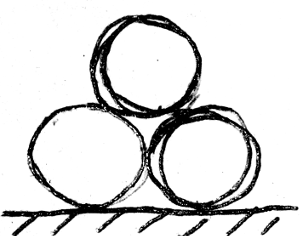
\includegraphics[width=3cm]{16}}
\task{17}{ Вася любит принимать ванну и знает, что для него комфортная температура воды 35$^\circ$C. К сожалению, у него на несколько дней отключили холодную воду. Вася померил температуру горячей воды, вытекающей из крана (60$^\circ$C), и заметил, что можно комфортно сидеть в набирающейся ванне, если каждые 7~секунд бросать в нее кубик льда из морозильника. На следующий день оказалось, что ледяные кубики приходится бросать каждые 5~секунд, хотя поток воды из крана такой же. На сколько изменилась температура воды в кране? Тепловыми потерями пренебречь, вода быстро перемешивается и кубики тают быстро.}

\end{document}